\documentclass[12pt,a4paper]{article}
\usepackage[utf8]{inputenc}
\usepackage[spanish]{babel}


% Paquetes

\usepackage{amsmath}
\usepackage{amsfonts}
\usepackage{amssymb}
\usepackage{amsthm}  % Permite crear teoremas nuevos / Estilos de teoremas 
\usepackage{graphicx} % 
\usepackage[colorlinks=true,allcolors=blue]{hyperref} % Crea las hiperreferencias (clicas y te mueves)
\graphicspath{ {Imagenes/} }
\usepackage{fancybox} % para usar la caja de los ejemplos
\usepackage{bigints } % permite crear grandes integrales
% Autor y titulo

\title{Apuntes Mecánica Clásica III}
\author{Daniel Vázquez Lago}

% Forma del  texto

\setlength{\parindent}{15px}
\usepackage[left=2.25cm,right=2cm,top=4cm,bottom=2cm]{geometry}

% Otros


\numberwithin{equation}{section}
\numberwithin{figure}{section}

% Comandos


\newcommand{\parentesis}[1]{\left( #1  \right)}
\newcommand{\parciales}[2]{\frac{\partial #1}{\partial #2}}
\newcommand{\pparciales}[2]{\parentesis{\parciales{#1}{#2}}}
\newcommand{\ccorchetes}[1]{\left[ #1  \right]}
\newcommand{\D}{\mathrm{d}}
\newcommand{\Dd}{\mathrm{D}}
\newcommand{\derivadas}[2]{\frac{\D #1}{\D #2}}
\newcommand{\sech}{\mathrm{sech} \ }
\newcommand{\csch}{\mathrm{csch} \ }
\newcommand{\cotanh}{\mathrm{cotanh}}
\newcommand{\cotan}{\ \mathrm{cotan}}
\newcommand{\Res}{\mathrm{Res}}
\newcommand{\Arg}{\mathrm{arg}}
\newcommand{\Real}{\mathrm{Re}}
\newcommand{\tquad}{\quad \quad \quad} 

\newcommand{\cte}{\ \mathrm{cte}}
\newcommand{\dete}{\ \mathrm{det}}
\newcommand{\Tr}{\ \mathrm{Tr}}

\newcommand{\rota}{\nabla \times}
\newcommand{\dive}{\nabla \cdot}

\newcommand{\vn}{\mathbf{v}}
\newcommand{\xn}{\mathbf{x}}
\newcommand{\Pn}{\mathbf{P}}
\newcommand{\pn}{\mathbf{p}}
\newcommand{\qn}{\mathbf{q}}
\newcommand{\Mn}{\mathbf{M}}
\newcommand{\Xn}{\mathbf{X}}
\newcommand{\Fn}{\mathbf{F}}
\newcommand{\gn}{\mathbf{g}}
\newcommand{\An}{\mathbf{A}}
\newcommand{\Sn}{\mathbf{S}}
\newcommand{\fn}{\mathbf{f}}
\newcommand{\en}{\mathbf{e}}
\newcommand{\un}{\mathbf{u}}
\newcommand{\neta}{\boldsymbol{\eta}}
\newcommand{\Ln}{\mathbf{L}}
\newcommand{\Nn}{\mathbf{N}}

\newcommand{\hnn}{\hat{\mathbf{n}}}
\newcommand{\hnr}{\hat{\mathbf{r}}}
\newcommand{\hnz}{\hat{\mathbf{z}}}
\newcommand{\hnx}{\hat{\mathbf{x}}}
\newcommand{\hny}{\hat{\mathbf{y}}}
\newcommand{\hnu}{\hat{\mathbf{u}}}
\newcommand{\hnR}{\hat{\mathbf{R}}}
\newcommand{\hnv}{\hat{\mathbf{v}}}

\newcommand{\Lcal}{\mathcal{L}}
\newcommand{\Hcal}{\mathcal{H}}
\newcommand{\Fcal}{\mathcal{F}}


\newtheorem{theorem}{Teorema}[section]
\newtheorem{corollary}{Corolario}[theorem]
\newtheorem{lemma}{Lema}[section]
\newtheorem{ejemplo}{Ejemplo}[section]
\newtheorem{definition}{Definicion}[section]
\newtheorem{proff}{Prueba}[lemma]



\begin{document}

\maketitle

\newpage

\tableofcontents

\newpage

\section{Formalismo Hamiltoniano}

\subsection{Hamiltoniano y Lagranino}

El estudio del movimiento de un cuerpo bajo un potencial se puede reducir al estudio de la acción. Según el \textit{principio de acción de Hamilton} todo cuerpo sigue una trayectoria tal que minimiza la acción. La acción es, básicamente, un funcional integral definido como:

\begin{equation}
S = \int_{t_1}^{t_2} \mathcal{L} (q, \dot{q}, t) \D t
\end{equation}

donde definimos $\Lcal$ como el \textbf{lagrangiano} del sistema que será la diferencia entre la energía cinética ($T$) y la energía potencial ($V$). La intención de esta integral es hallar la función $q(t)$ que minimice la acción. Para esto se tiene que verificar la siguiente ecuación diferencial de segundo orden llamada la \textbf{ecuación de Euler-Lagrange}:

\begin{equation}
\derivadas{}{t} \parentesis{\parciales{\Lcal}{\dot{q}}} - \parciales{\Lcal}{q} = 0 \label{Ec:1.0-Eu-La}
\end{equation}

Para $N$ coordenadas tendremos $N$ ecuaciones de Euler-Lagrange. Hamilton desarrollo una función análoga al lagrangiano llamada el \textbf{Hamiltoniano} $\Hcal$. Esta función es la transformada de Legendre del lagrangiano, y se escribe en función de los momentos, no de las velocidades. Definimos momento de una coordenada $x_j$ como:

\begin{equation} 
p = \parciales{\Lcal}{\dot{q}} \label{Ec:1.0-p}
\end{equation}
Si substituimos esto en la ecuación \ref{Ec:1.0-Eu-La}, tenemos que

\begin{equation}
\dot{p} = \parciales{\Lcal}{q}  \label{Ec:1.0-pdot}
\end{equation}
la cual será muy interesante posteriormente. La definición de Hamiltoniano vendrá dada por:

\begin{equation}
\Hcal(q,p,t) = p \dot{q} - \Lcal(q,\dot{q},t)
\end{equation}
Una vez obtuvimos el Hamiltoniano tenemos que encontrar la ecuación de segundo orden análoga a la ecuación de Euler-Lagrange. En este caso lo que tendremos en realidad serán dos ecuaciones de primer orden, muy fácilmente deducibles, tal y como presentaremos a continuación. A las ecuaciones que resuelven las ecuaciones de movimiento para el Hamiltoniano

\begin{equation}
\dot{q} = \parciales{\Hcal}{p}; \quad \dot{p} = - \parciales{\Hcal}{q}; \quad 
\derivadas{\Hcal}{t} = \parciales{\Hcal}{t} = - \parciales{\Lcal}{t}
\end{equation}
siendo una de las propiedades del Hamiltonioan que su única dependencia con el tiempo es la dependencia explícita. Si no aparece de manera explícita el Hamiltoniano será constante en el tiempo. Estas condiciones son sencillas de obtener si nos fijamos que

\begin{equation}
\D \Lcal = \pparciales{\Lcal}{t} \D t +  \pparciales{\Lcal}{q} \D q +  \pparciales{\Lcal}{\dot{q}} \D \dot{q}
\end{equation}
Usando las definiciones \ref{Ec:1.0-p} y \ref{Ec:1.0-pdot} en la ecuación anterior, y substituyéndolas en el hamiltoniano
$$
\D \Hcal = \dot{q} \D p + p  \D \dot{q} - \D \Lcal = \dot{q} \D p - \dot{p} 
$$
obtenemos que

\begin{equation}
\Hcal = \dot{q} \D \dot p - \dot{p} \D q  - \pparciales{\Lcal}{t} \D t
\end{equation}
De donde lógicamente obtenemos las ecuaciones canónicas. 

\subsection{Transformaciones Canónicas}

Definimos una \textbf{transformación canónica} como una transformación (cambio de variables) del espacio de fases que mantenga las ecuaciones de Hamilton. En otras palabras, es un cambio de variables que nos permite escribir las ecuaciones de otra manera, sin pérdida de información de ningún tipo. Si el espacio de fases inicial es $(q_i,p_i) \ i = 1,2...n$, una transformación canónica tendrá la siguiente forma funcional:

\begin{equation}
Q = Q (q_i,p_i,t); \quad P = P (q_i,p_t,t) \quad i = 1,2,...n
\end{equation}
pudiendo tener una dependencia de todas las coordenadas del espacio de fases inicial. Lógicamente si tenemos $2N$ coordenadas ($N$ espaciales, $N$ momentos) tendremos que hacer $2N$ cambios para transformar todo el espacio de fases, aunque podemos limitarnos a transformar solo algunas coordenadas. \\

Las ecuaciones del movimiento de ambos espacios de fases deben ser completamente análogas, sin embargo está claro que la Hamiltoniana $\Hcal(q_i,p_i,t)$ tendrá otra forma funcional tal que $K(Q_i,P_i,t)$; y lo mismo para las ecuaciones: la forma explícita puede ser otra, pero no puede cambiar la naturaleza de las mismas. A partir de una podemos recuperar la otra. El hamiltoniano de las nuevas coordenadas lógicamente verificará las ecuaciones canónicas:
 
\begin{equation}
\dot{Q_i} = \parciales{K}{P_i}; \quad \dot{P_i} = - \parciales{K}{Q_i} \quad i =1,2,...n \label{Ec:1.1-Ecuaciones-canonicas-K}
\end{equation}

Antes de continuar debemos comprender un momento cual es el interés de esto. Muchas veces tenemos problemas realmente difíciles de solucionar mediante las coordenadas originales (pensemos por ejemplo en tratar en resolver la ecuación de un oscialador armónico en coordenadas cartesianas). Ser capaz de encontrar unas nuevas variables para las cuales las ecuaciones diferenciales son mucho mas sencillas de resolver es una parte fundamental del estudio de la física, y que dicho cambio nos de la misma solución es vital. Entonces se hace necesario saber cual puede ser la relación entre las hamiltonianas o las variables para que el cambio conserve el movimiento del cuerpo (ecuaciones del movimiento análogas). \\

Deducir la relación entre las hamiltonianas es bastante sencillo, ya que para que se verifique es suficiente que las funciones $H$ y $K$ difieran en una derivada parcial de una función $F$ tal que:

\begin{equation}
K = H + \derivadas{F}{t} \label{Ec:1.1-K-H}
\end{equation}

Esto es porque dicha derivada deja invariante a la acción de Hamilton, y por tanto a las ecuaciones de movimiento. Intuitivamente uno puede ver que dicho cambio en la acción de Hamilton deja invariante la ecuación ante cambios infenitesimales, ya que

\begin{equation}
\delta S = \int_{t_1}^{t_2} \D t \ccorchetes{p_i \dot{q}_i - H} = \int_{t_1}^{t_2} \D t \ccorchetes{P_i \dot{Q}_i - K + \dfrac{\D F}{\D t}} 
\end{equation}

tal que este último término tiende a cero cuando el cambio es infenitesimal, y por lo tanto, obliga a que se verifiquen las ecuaciones \ref{Ec:1.1-Ecuaciones-canonicas-K}. En otras palabras debe verificarse que:

\begin{equation}
p_i \dot{q}_i - P_i \dot{Q}_i - H + K + \dfrac{\D F}{\D t} = 0 \label{Ec:1.1-K-H2}
\end{equation}


 A la función $F(q_i,p_i,Q_i,P_i,t)$ se llama \textbf{función generatriz de la transformada canónica}. Es obvio que su dependencia es de $2N$ coordenadas, ya que ellas  son mutuamente dependientes. Si por ejemplo solo tuviéramos un grado de libertad de tal modo que $F(q,p,Q,P,t)$ tendríamos que solo dependería de 2 variables, ya que sabemos que existe dos ecuaciones que parametrizan $Q$ y $P$ respecto $q$ y $p$. La forma funcional de $F$ tiene entonces que ser:

\begin{equation}
F = F_1 (q,Q,t)
\end{equation}
\begin{equation}
F = F_2 (q,P,t)
\end{equation}
\begin{equation}
F = F_3 (p,Q,t)
\end{equation}
\begin{equation}
F = F_4 (p,P,t)
\end{equation}
a partir de ellas haremos nuestro cambio de coordenadas canónicas, y por tanto a partir de ellas podremos construir una nuevas ecuaciones con diferentes, que, idealmente, serán mas sencillas de resolver que las originales. Por ejemplo, si somos capaces de encontrar una $F$ para la cual $K$ es cero tendríamos que todas las coordenadas del nuevo sistema de fases serían cíclicas, resolviendo directamente el sistema sin hacer una sola ecuación o integral. \\

Si conocemos una función generatriz de la transformada canónica podremos hacer directamente el cambio de coordenadas ya que se verificará que:
 
\begin{itemize} 
\item $\mathbf{F_1}$:
\begin{equation}
p_i = \parciales{F_1}{q_i}; \quad P_i = - \parciales{F_1}{Q_i} \label{Ec:1.1-piF1}
\end{equation} \\

\item $\mathbf{F_2}$:
\begin{equation}
p_i = \parciales{F_2}{q_i}; \quad Q_i = \parciales{F_2}{P_i} \label{Ec:1.1-piF2}
\end{equation} \\

\item $\mathbf{F_3}$:
\begin{equation}
q_i = - \parciales{F_3}{p_i}; \quad P_i = - \parciales{F_3}{Q_i} \label{Ec:1.1-piF3}
\end{equation}\\

\item $\mathbf{F_4}$:
\begin{equation}
q_i = - \parciales{F_4}{p_i}; \quad Q_i =  \parciales{F_4}{P_i} \label{Ec:1.1-piF4}
\end{equation}
\end{itemize}

El lector ahora mismo debe estar pensando que esto sale de la nada. Quizás uno que quiera tener una chuleta puede serle suficiente, pero aquí presentaremos cual es la fórmula para llegar a estas ecuaciones, de tal modo que podamos deducir cuales son para las otras $F$. Entonces si:

\begin{equation}
\dfrac{\D F_1}{\D t} = \dfrac{\partial F_1}{\partial q} \dot{q} + \dfrac{\partial F_1}{\partial Q} \dot{Q} 
\end{equation}
tal que si lo substituimos en la ecuación \ref{Ec:1.1-K-H} podemos ver que:
\begin{equation}
K = H + \dfrac{\D F_1}{\D q} \dot{q} + \dfrac{\partial F_1}{\partial Q} \dot{Q}  \longrightarrow K - \dfrac{\partial F_1}{\partial Q} \dot{Q}  = H + \dfrac{\partial F_1}{\partial q} \dot{q} 
\end{equation}
y si dichas relaciones las metemos dentro de la ecuación \ref{Ec:1.1-K-H2} vemos que solo se verifica la igualdad si se verifican las ecuaciones \ref{Ec:1.1-piF1}. Además esto nos lleva a deducir que las relaciones entre las funciones generatrices y $F_1$ es una \textit{transformada de Legendre}, siendo estas relaciones entre funciones:

\begin{equation}
F_2(q,P,t) = F_1 - Q \parciales{F_1}{Q} = F_1 + QP
\end{equation}
\begin{equation}
F_3(q,P,t) = F_1 - q \parciales{F_1}{q} = F_1 - q p
\end{equation}
\begin{equation}
F_4(q,P,t) = F_1 - q \parciales{F_1}{q} - Q \parciales{F_1}{Q} = F_1 - qp + QP 
\end{equation}

Existen entonces dos tipos de problema a los que nos podamos enfrentar. El primero de ellos será cuando nos den una función generatriz cualquiera, y a partir de ella tendremos que deducir cual ha sido el cambio de coordenadas, calcular las otras funciones generatrices posibles... Para esto último podemos tomar dos vías: usar la transformada de legendre o derivar el cambio de coordenadas y luego integrar usando las diferentes ecuaciones \ref{Ec:1.1-piF1}, \ref{Ec:1.1-piF2}, \ref{Ec:1.1-piF3} o \ref{Ec:1.1-piF4}. \\

El otro tipo de problema implicará conocer la transformada canónica, y tener que calcular las funciones generatrices mediante integrales y transformada de Legendre. Sin embargo el lector no debe ser ingenuo: antes de realizar dichas integrales debe saber si el cambio es realmente canónico. Para saber si es una transformada canónica usaremos los recursos dados en los dos siguientes puntos: la forma matricial y los corchetes de Poisson. 


\subsection{Forma matricial de las tranformaciones canónicas}

Supongamos que tenemos $2n$ coordenadas que escribimos de manera vectorial tal que $\vec{q}=(q_1,q_2,\ldots,q_n)$ y $\vec{p} = (p_1,p_2,\ldots,p_n)$. Considerando que nuestro espacio de fases será $\vec{x} = (\vec{q}, \vec{p})$; podemos buscar otro espacio de fases formado por $\vec{y} = (\vec{P},\vec{Q})$ de $2n$ componentes de tal modo que se verifique una relación:

\begin{equation}
\vec{y} = \vec{y} (\vec{x}) 
\end{equation}

tal que cada una de las componentes de $\vec{y}$ depende de $\vec{x}$. Ahora bien, uno podría preguntarse el porqué de todo esto, y la respuesta no podría ser mas sencilla. En primer lugar estamos generalizando a un caso con $2n$ coordenadas y por lo tanto generalizamos el estudio para un sistema con los grados de libertad que queramos. La utilidad es bien clara. Si somos capaces de desarrollar un método para el cual encontremos una función generatriz de manera general, o estudiar si es posible dicha transformación habremos desarrollado una herramienta muy potente para estudiar la dinámica de los sistemas. \\

El conocimiento de matrices y álgebra lineal es fundamental para el estudio de este temario. Si se comprende bien el álgebra básica será muy sencillo para el lector entender lo que viene a continuación. Derivando la relación respecto al tiempo es muy fácil de ver que:

\begin{equation}
\dot{y}_a = \parentesis{\parciales{y_a}{x_b}} \dot{x_b}
\end{equation}

Podemos sin ningún tipo de dudas definir una matriz jacobiana $\Mn$ para dicha transformación, de tal modo que cada elemento de la matriz viene definido por:

\begin{equation}
M_{ab} =  \parentesis{\parciales{y_a}{x_b}} 
\end{equation}
Ahora bien queremos encontrar cual es la condición necesaria y suficiente para demostrar que dicha transformación del espacio de fases es canónica y por lo tanto deja al sistema como un sistema hamiltoniano. Sea $\mathbb{J}$ una \textbf{matriz simpléctica}. Definimos la matriz simpléctica como una matriz $2n \times 2n $ tal que:

\begin{equation}
\mathbb{J}_{2n \times 2n} = \begin{pmatrix}
0_{n \times n} & \mathbb{I}_{n \times n} \\
\mathbb{I}_{n \times n} & 0_{n \times n}
\end{pmatrix}
\end{equation}
siendo $\mathbb{I}$ la matriz identidad y $0$ la matriz cero. El valor $n$ corresponderá al número de grados de libertad del sistema (recuérdese que para cada grado de libertad tenemos dos coordenadas en el espacio de fases, una posicion y un momento). En ese caso \textit{la condición necesaria y suficiente} para que una transformación sea canónica es que:

\begin{equation}
\Mn \cdot \mathbb{J} \cdot \Mn^T = \mathbb{J}
\end{equation}

Como se define una matriz con forma simpléctica aquella que deja invariante la forma simpléctica podemos decir que la condición para la trasformación sea canónica es que la matriz $\Mn$ sea simpléctica. Esta condición tan complicada puede ser bastante pesada de usar, sobretodo si tenemos un espacio de fases muy grandes. La siguiente parte estudiará una forma mucho mas sencilla para verificar las trasformadas canónicas, mucho mas sencilla y poderosa.

\subsection{Corchetes de Poisson}

Los corchetes de Poisson son una herramienta súper útil a la hora de encontrar transformadas canónicas para nuestro problema. Sea $F$ y $G$ dos funciones del espacio de fases dependientes del tiempo tal que $F=(q_i,p_i,t)$ y $G=(q_i,p_i,t)$, definimos como \textbf{corchete de Poisson} al siguiente operador:

\begin{equation}
\{ F,G \} = \sum_{i=1}^n \parentesis{\parciales{F	}{p_i}\parciales{G}{p
q_i}-\parciales{F}{q_i}\parciales{G}{p_i}}
\end{equation}
que tendrá las siguientes propiedades:

\begin{itemize}
\item Antisimetría: $\{ F,G \} = - \{ G,F \}$
\item Bilinealidad: $\{ \alpha A + \beta B, C \} = \alpha \{A,C\} + \beta \{B,C\}$
\item Derivación: $\{AB,C \} = A\{ B,C \}+ B \{ A,C \}$
\end{itemize}

Todas estas propiedades son fundamentales a la hora de resolver ejercicios, rogamos al lector que las aprenda y no las dude, le facilitará mucho el cálculo de trasformadas canónicas y estudio de las ecuaciones del movimiento. Los pasos para demostrar estas son triviales, a fin de cuentas los corchetes de poisson no dejan de ser una suma de derivadas y por tanto hereda la mayoría de las propiedades de las derivadas. La única propiedad que no verifica es la propiedad asociativa. \\

Los casos particulares para las coordenadas $p,q$ de tal modo que:

\begin{equation}
\{ q_i, q_ j \} = \{ p_i , p_j \} = 0 \quad \quad \{q_i,p_j\} = \delta_{ij}
\end{equation}
\begin{equation}
\{ q_i, F \} = \parciales{F}{p_i} \quad \quad \{ p_i, F \} = - \parciales{F}{q_i}
\end{equation}

Los siguientes teoremas deben tenerse muy ensomos capaces de  cuenta a la hora de resolver ejercicios. Las implicaciones de estos serán tratados después de enunciarlos:

\begin{theorem}
una transformación en el espacio de fases es canónica si y solo si deja invariantes a los chorchetes de Poisson fundamentales.
\end{theorem}

Es decir, tenemos que las funciones $P$ y $Q$ deben verificar, para que sean transformaciones canónicas, las siguientes relaciones:

\begin{equation}
\left\lbrace Q , P \right\rbrace_{q,p} = 1 
\end{equation}

\begin{theorem}
los corchetes de Poisson son invariantes bajo transformaciones canónicas.
\end{theorem}

Este último tiene gran utilidad, ya que nos dice que si tenemos dos funciones $F$ y $G$ definidas en el espacio de fases $q_i,p_i$, y las expresamos en un nuevo espacio de fases a través de una función generatriz $Q_i, P_i$ tenemos que se verifica que:


\begin{equation}
\{ F(q_i,p_i,t), G(q_i,p_i,t) \} = \{ F(Q_i,P_i,t), G(Q_i,P_i,t) \}  
\end{equation}


\subsection{Evolución temporal}

Se puede demostrar fácilmente que la dependencia temporal de una función $F$ del espacio de fases cualquiera verifica que:

\begin{equation}
\derivadas{F}{t} = \parciales{F}{t} + \{ F, H \}
\end{equation}

siendo $H$ la Hamiltoniana. En este formalismo será condición suficiente para que una función $F$ sea constante que su corchete de Poisson respecto el Hamiltoniano sea cero y que no tenga el tiempo como función explícita. Es decir si:

\begin{equation}
\{ F, H \} = 0; \quad \parciales{F}{t} = 0 \Longrightarrow F = \cte
\end{equation}
de esto precisamente se deduce el siguiente teorema, llamado \textbf{teorema de Poisson}, que nos ayuda a encontrar nuevas constantes del movimiento a partir de dos conocidas. 

\begin{theorem}[Teorema de Poisson]
si dos funciones $F,G$ del espacio de fases son constantes del movimiento, su corchete de Poisson es también una constante del movimiento.
\end{theorem}

Se deduce entonces que si $F=G=H$ (Hamiltoniana), entonces por ser $\{ F, G \} = \{ H, H \} = 0$, tendremos que 

\begin{equation}
\derivadas{H}{t} = \parciales{H}{t}
\end{equation}
tal y como ya sabíamos.


\subsection{Teoría de Hamilton-Jacobi}

\subsubsection{Ecuación principal de Hamilton}

Podemos asegurar que las nuevas variables canónicas son constantes si nuestra nueva hamiltoniana es $K=0$ de tal modo que

\begin{eqnarray}
\parciales{K}{P_i}  = \dot{Q}_i = 0 \\
- \parciales{K}{Q_i}  =  \dot{P}_i = 0
\end{eqnarray}
Como se ha visto podemos relacionar $K$ con $H$ y una función generatriz $F$ (ecuación \ref{Ec:1.1-K-H}). En ese caso la función $F$ satisface la ecuación:

\begin{equation}
\parciales{F}{t} = - H (q,p,t) \label{Ec:1.42}
\end{equation}
Usaremos la función $F_2(q,P,t)$, ya que nos interesa usar las coordenadas de posición $q_i$ y la nueva constante de momento. COmo sabemos se verifica que

$$ p_i = \parciales{F_2}{t} $$
Dado que el hamiltoniano es una función explícita de $q$, $p$ y $t$ ; tendremos que la ecuación \ref{Ec:1.42} se puede escribir como 

\begin{equation}
H \parentesis{q_i, \parciales{F_2}{q_i};t} + \parciales{F_2}{t} = 0
\end{equation}
que llamaremos \textbf{ecuación de Hamilton-Jacobi}. A la función $F_2$ la denotaremos a partir de ahora $S$, y la llamaremos como \textbf{función principal de Hamilton}. Por supuesto la integral de dicha ecuaciónsolo demuestra la dependencia en las  viejas coordenadas y del tiempo, no aparecerán los nuevos momentos $P_i$, aunque sean constantes (como es evidente). \\

Matematicamente la ecuación es una ecuación diferencial ordinaria de primer orden en n+1 variables. Supongamos que existe una solución de la forma

$$ S = S(q_1,...,q_n;\alpha_1,...,\alpha_{n+1};t) $$
donde las constantes $\alpha_i$ son constantes de integración independientes. En cualquier caso existe una constante que es irrelevante, ya que si $S$ es solución, $S+\kappa$ también es solución, por lo que 

\begin{equation}
 S = S(q_1,...,q_n;\alpha_1,...,\alpha_{n};t) 
\end{equation}
Lógicamente podemos asociar estas $n$ constantes de integración con los $n$ momentos:

\begin{equation}
P_i = \alpha_i
\end{equation}
Ahora el momento

\begin{equation}
p_i = \parciales{S(q,\alpha,t)}{q_i}
\end{equation}
Por otro lado las constantes $Q_i$ también se pueden calcular a partir de $S$ como:

\begin{equation}
Q_i = \beta_i = \parciales{S(q,\alpha,t)}{\alpha_i}
\end{equation}
Las constantes $\beta$ se pueden obtener simultáneamente a partir de las condiciones iniciales. Así podremos obtener, tras despejar, los valores de $q_j$ y $p_j$ en función de las constantes ($\alpha,\beta$) y el tiempo ($t$). \\

Así cuando resolvemos la ecuación de Hamilton-Jacobi, estamos al mismo tiempo obteniendo la solución al problema mecánico. Matematicamente hemos establecido la equivalencia entre las $2n$ ecuaciones canónicas (2n ecuaciones de primer orden) con una ecuación de primer orden en derivadas parciales. Podemos ver que la derivada temporal de la función principal de Hamilton nos lleva a la fórmula

$$ \derivadas{S}{t} = \parciales{Q}{q_i} \dot{q}_i + \parciales{S}{t} $$
ya que $P_i$ son constantes. Esta relación se puede escribir como

\begin{equation}
\derivadas{S}{t} = p_i \dot{q}_i + \parciales{S}{t} = L
\end{equation}
por lo que la función prinicpal de Hamilton se puede entender como la acción mas una constante. Sin embargo esta función no es útil a la hora de calcular $S$ ya que para resolver la integral

\begin{equation}
S = \int L \D t + \text{constante}
\end{equation}
necesitamos conocer $q$ y $p$ como funciones explícitas del tiempo, y ese es precisamente el problema que queremos resolver. \\

Resolvamos un caso sencillo y bastante común, que es el hamiltoniano no dependiente explícitamente del tiempo, de tal modo que $H$ es una constante. Cuando esto es así podremos separar variables de tal modo que si $H=E=\alpha$ tenemos que $S$ solo puede venir dado por

\begin{equation}
S ( q,\alpha,t) = W(q,\alpha) - \alpha t
\end{equation}
donde $W(q,\alpha)$ es llamada la \textbf{función característica de Hamilton}. El significado físico de $W$ peude entenderse cuando escribimos su derivada respecto al tiempo

\begin{equation}
\derivadas{W}{t} = \parciales{W}{q_i} \dot{q}_i
\end{equation}
Dado que 

\begin{equation}
\parciales{S}{q_i} = \parciales{W}{q_i} = p_i
\end{equation}
de tal modo que 

\begin{equation}
\derivadas{W}{t} = p_i \dot{q}_i
\end{equation}

\subsubsection{El oscilador armónico como ejemplo}


\subsubsection{Función característica de Hamilton}

Es posible obtener la solución de los problemas usando separación de variables siempre que $H$ no dependa explícitamente del tiempo, de tal modo que $H=E=\alpha$ es una constante del tiempo. Cuando esto ocurre, l ecuación característica de Hamilton independiente del tiempo $W$ aparece de manera explícita en el cálculo de $S$. De hecho, esta función $W$ genera una transformación canónica propia. \\

Consideremos entonces la transformación canónica a partir la cual todos los momentos $P$ son constantes del movimiento $\alpha_i$, y donde $\alpha_1$ es, en particular, la constante de movimiento $H$. Denotando a esta función generatriz como $W(q,P)$ tal que

\begin{equation}
p_i = \parciales{W}{q;i} \tquad Q_i = \parciales{W}{P_i}=\parciales{W}{\alpha_i}
\end{equation}
dado que $W$ no depende explícitamente del tiempo, la nueva y la vieja hamiltoniana son iguales, de tal modo que $K=\alpha_1$. \\

La función característica de Hamilton $W$ en este caso genera una transformación canónica donde todas las coordenadas son cíclicas. En este caso: 

\begin{equation}
\dot{P}_i = - \parciales{K}{Q_i} = 0 \tquad P_i = \alpha_i
\end{equation}
Dado que la nueva hamiltoniana depende únicamente del momento $\alpha_1$, tenemos que

\begin{equation}
\dot{Q}_i = \parciales{K}{t} = \left\lbrace \begin{array}{ll}
1 & i=1\\
0 & i \neq 1 
\end{array} \right.
\end{equation}
En el caso de que no tomemos $P_1=\alpha_1=H$, de tal modo que $P_i = \gamma_i$, podremos ver que:


\begin{equation}
\dot{Q}_i = \parciales{K}{\gamma_i} =v_i
\end{equation}
tal que

\begin{equation}
Q_i = v_i t + \beta_i 
\end{equation}


\subsection{Integrabilidad}

\begin{definition}[Sistema integrable]
un sistema hamiltoniano conservativo con $n$ grados de libertad se llama \textit{integrable} si existen $n$ cantidades conservadas, es decir, existen $F_i$, $i=1,2...n$ tal que:
\begin{itemize}
\item $\{ F_i , H \} = 0, \ \forall i$
\item $\{ F_i , F_j \} = 0, \ \forall i,j$
\item Vectores $\nabla F_i$ linealmente independientes.
\end{itemize}
\end{definition}
 
\begin{theorem}[Lioville-Arnold]
si un sistema hamiltoniano es integrable con $n$ grados de libertad tal que el sistema de fases es $(q_i,p_i) i = 1,2...n$ tenemos que:
\begin{itemize}
\item Existen variables canónicas tales que $(\phi_i,\ldots,\phi_n,J_1,\ldots,J_)$ podemos encontrar una hamiltoniana tal que $H=H(J_1,\ldots,J_n)$, tal que las ecuaciones del movimiento son:
\begin{equation}
J_i = c_i \tquad \phi_i = w_i t + \phi_i
\end{equation}
\item Las ecuaciones canónicas en las variables originales se pueden resolver separando variables e integrando.
\end{itemize}
\end{theorem}


\newpage

\section{Sistemas non lineales y dinámica en el espacio de fases}

La mayor parte de los sistemas mecánicos no son solucionables analíticamente, es decir, no podemos encontrar unas funciones que nos describan fielmente su comportamiento. Esto por ejemplo puede ocurrir cuando tenemos mas ecuaciones que constantes del movimiento (problema de los 3 cuerpos bajo atracción gravitacional mutua), por lo que sería imposible predecir, con unas condiciones de frontera o contorno dadas, la posición de los cuerpos en un tiempo $t$ que queramos. En este tema desarrollaremos una teoría que nos permita estudiar el comportamiento de sistemas dinámicos no gobernados por una hamiltoniana, con dos métodos: teoría de perturbaciones y geometría del espacio de fases. 

\subsection{Teoría de Perturbaciones}

La teoría de perturbaciones nos permite resolver numéricamente ciertos problemas que analíticamente no son resolubles. La idea es aproximar el problema a uno similar pero resoluble. La base de dicha teoría es introducir ciertos parámetros pequeños de tal manera que podamos substituir numéricamente estos para que las soluciones se parezcan lo máximo posible a la realidad. En este apartado nos limitaremos a estudiar algunos de sus ejemplos.

\subsection{Sistemas Dinámicos}

Sean $x_1,x_2,...,x_n$ un conjunto de variables dinámicas que pueden representar gran variedad de magnitudes como posición, velocidad, momento, poblaciones de individuos... Entonces el estado de nuestro sistema vendrá dado por un \textit{vector} o \textit{punto en el espacio de fases} tal que $\xn = (x_1,x_2,...x_N)$. Todos los sistemas que consideremos serán sistemas deterministas, en los que la evolución temporal completa viene determinado por los valores iniciales. Definimos $\Fn$ como el \textit{campo vectorial} o \textit{campo de velocidades} es:

\begin{equation}
\derivadas{\xn(t)}{t} = \Fn (\xn(t),t)
\end{equation}

Además pueden existir parámetros $\lambda$ llamados \textit{parámetros de control} que afectan a la dinámica (masas, cargas, frecuencias...). Si $\Fn$ depende explicitamente de $t$ decimos que es un \textit{sistema no autónomo}. Si $\Fn$ no depende explicitamente de $t$ decimos que el sistema es un \textit{sistema autónomo}. \\

\subsubsection{Sistemas Dinámicos Hamiltonianos}

Si nuestro sistema de fases son $n$ coordenadas espaciales y $n$ coordenadas de momento tal que $\xn = (\qn,\pn)$. En ese caso las ecuaciones canónicas pueden escribirse como:

\begin{equation}
\dot{\xn} = \mathbb{J} \cdot \vec{\nabla}_x H = \mathbb{J} \cdot \parciales{H}{\xn}
\end{equation}
Trataremos al vector $\dot{\xn}$ como un sistema dinámico $\Fn(\xn,t)$, de tal manera que cada componente de dicho sistema será:

\begin{equation}
F_i (\xn,t) = J_{ij} \parciales{H}{x_j}
\end{equation}
siendo $\mathbb{J}$ la matriz simpléctica. Definimos la matriz simpléctica como una matriz $2n \times 2n $ tal que:

\begin{equation}
\mathbb{J}_{2n \times 2n} = \begin{pmatrix}
0_{n \times n} & \mathbb{I}_{n \times n} \\
\mathbb{I}_{n \times n} & 0_{n \times n}
\end{pmatrix}
\end{equation}
tal que $\mathbb{I}$ es la matriz identidad y $0$ es la matriz ceros (todo cero).
\subsubsection{Trayectorias, órbitas y flujos}

El estudio de los sistemas dinámicos incluye el estudio de diagramas de fase, como el siguiente:

\begin{figure}[h!] \centering
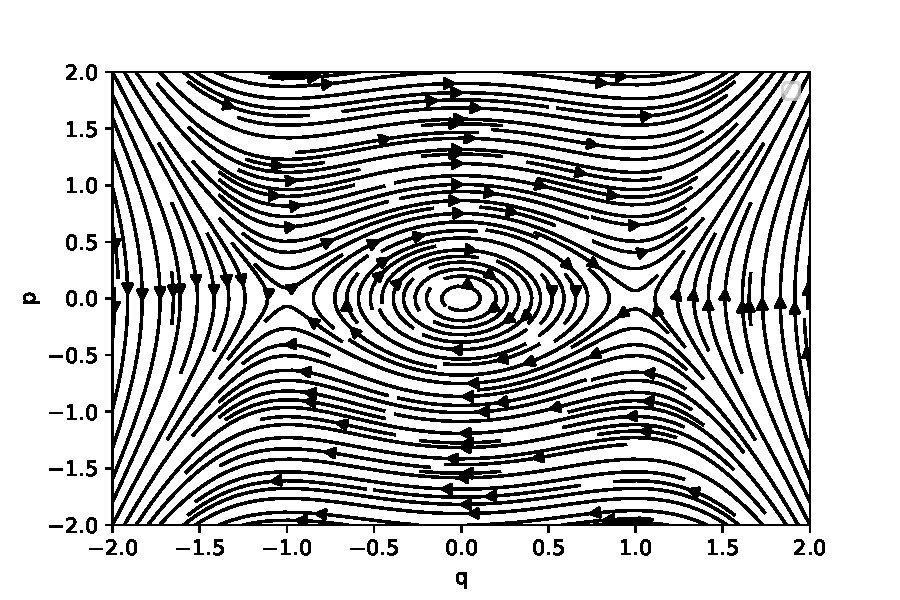
\includegraphics[scale=1]{Ejercicio-23a.pdf}
\end{figure}

Un sistema dinámico nos permite, conocido el hamiltoniano y un punto, la trayectoria en el espacio de fases que seguirá el cuerpo (no conoceremos  cuanto tiempo se demora de un punto a otro...). Entones cada punto del dominio del espacio de fases actúa como una condición inicial, y las soluciones como curvas parametrizadas por el tiempo $t$, llamadas \textit{órbitas} o \textit{trayectorias}. Para sistemas autónomos podemos obtener información sobre la naturaleza general de las trayectorias sin necesidad de calcularlas explícitamente. 

\begin{theorem}
por cada punto del espacio de fases de un sistema autónomo pasa una trayectoria y solo una.
\end{theorem}

Esto implica que en un sistema autónomo las trayectorias de fases no se cruzan. Si gráficamente vemos que 4 lineas ``coinciden'' lo mas probable es que dichas trayectorias mueran en dicho punto del espacio de fase. Véase el espacio de fases presentado arriba, donde ciertas líneas convergen a ciertos puntos. En verdad no se cruzan en dicho punto, si no que mueren alli ($\vec{F} = (0,0)$ en dicho punto). Esto implica que los movimientos periódicos corresponden a curvas cerradas simples; y que las curvas cerradas simples corresponden a movimientos periodicos. \\

Ahora presentaremos una de las partes mas importantes del estudio de los sistemas dinámicos: la teoría de la estabilidad.

\subsubsection{Teoría de la estabilidad}

Vamos a estudiar la estabilidad en los sistemas dinámicos, de tal manera que podamos conocer el comportamiento general del sistema, y poder conocer cual es la estabilidad de los sistemas dinámicos sin necesidad de conocer las soluciones explicitamente.  \\

En dicho proceso podremos conocer con muchísima precisión el comportamiento cerca de los \textit{puntos de equilibrio}. Por ejemplo el estudio del péndulo simple requiere una aproximación a pequeñas perturbaciones, de tal manera que conocemos con exactitud cual es el comportamiento cerca del punto de equilibrio. No obstante, fuera de dicho rango no conocemos analíticamente el problema. Similar a esto empezamos definiendo los \textit{puntos de equilibrio} y los \textit{tipos de punto de equilibrio}.


\begin{definition}[punto de equilibrio]
Definimos \text{punto de equilibrio} como aquel punto del espacio de fases $\xn_q$ tal que:

\begin{equation}
\Fn (\xn_q,t)= 0  \ \ \forall t
\end{equation}
\end{definition}

\begin{definition}[punto de equilibrio estable]
Sea $\xn(t_0) = \xn_0$ un punto inicial próximo al punto $x_q$. Definimos \text{punto de equilibrio estable} como aquel punto $x_q$ que cumple que:

\begin{equation}
\forall \epsilon > 0 \ \ \ \ \exists \delta (e) > 0 \ | \  \Vert \xn_0 - \xn_q \Vert < \delta \Longrightarrow \ \Vert \xn (t) - \xn_q \Vert < \epsilon, \ \forall t >  t_0
\end{equation}
\end{definition}

\begin{definition}[punto de equilibrio asintoticamente estable]
Sea $\xn (t_0) = \xn_0$ un punto inicial próximo a $\xn_q$. Entonces $\xn_q$ es un \text{punto de equilibrio asintoticamente estable} si:

\begin{equation}
\exists \delta > 0 \ | \ \Vert \xn_0 - \xn_q \Vert
 < \delta \Longrightarrow \lim_{t \rightarrow \infty} \Vert \xn (t) - \xn_q \Vert = 0
\end{equation}
\end{definition}

Podemos extender el concepto de soluciones estables apoyándonos en las definiciones de puntos de equilibrio. Entonces sea una solución $\xn^* (t) = \xn^* (t,\xn_0^*)$ con condición inicial $\xn_0^*$. Consideremos otra solución $\xn (t) = \xn (t,\xn_0)$ con condición inicial $\xn_0 = \xn (t_0)$. En este marco formulamos las siguientes definiciones:

\begin{definition}[solución estable]
Decimos que una solución $\xn^*(t)$ es estable siempre que se verifique que:
\begin{equation}
\forall \epsilon > 0 \ \ \exists \delta(\epsilon)> 0 \ | \ \Vert \xn (t_0) - \xn^*(t_0) \Vert < \delta \Longrightarrow \Vert \xn (t) - \xn^* (t) \Vert < \epsilon, \ \forall t > t_0
\end{equation}
\end{definition}


\begin{definition}[estabilidad asintótica de las soluciones]
la solución $\xn^* (t)$ es asintoticamente estable si las trayectorias convergen:
\begin{equation}
\exists \delta > 0 \ | \ \Vert \xn(t_0) - \xn^* (t_0) \Vert < \delta \Longrightarrow \lim_{t \rightarrow \infty} \Vert \xn(t)  - \xn^* (t) \Vert = 0
\end{equation}
\end{definition}


\subsubsection{Aproximación lineal}

La aproximación lineal estudia las proximidades de los puntos de equilibrio, clasificando dichos puntos en función de las relaciones lineales de primer orden cerca de dicho punto. Supongamos que en las cercanías al punto crítico la función $\neta$ definida como:

\begin{equation}
\neta (t) = \xn (t) - \xn^*
\end{equation}
será muy pequeña. Entonces podemos expresar la forma funcional como:

\begin{equation}
\dot{\neta}(t) = \dot{\xn} = \Fn (\xn,t) = \Fn (\xn^*,t) + \left. \derivadas{\Fn}{\xn} \right|_{\xn = \xn ^*} + \cdots
\end{equation} 
tal que la derivada de $\Fn$ es una matriz jacobiana expresada en adelante como $\An$  en el punto $\xn^*$ y $\eta(t)=\xn-\xn^*$ (pudiendo ser compleja). Ello implica que:

\begin{equation}
\derivadas{\neta (t)}{t} = \An \cdot \neta (t)
\end{equation}

 En general los elementos de $\An$ serán dependientes del tiempo salvo en sistemas autónomos para los cuales es una matriz de coeficientes constantes. \\

\begin{equation}
\An = \left. \dfrac{\D \Fn(\xn,t)}{\D \xn} \right|_{\xn^*} \tquad A_{ij} = \left. \dfrac{D F_i}{x_j} \right|_{\xn^*}
\end{equation}

Teniendo en cuenta además que dicha matriz relaciona de manera unequívoca el campo de velocidades y el campo de posiciones en las proximidades de dicho punto:

\begin{equation}
\Fn(\xn,t) = \An \cdot \xn
\end{equation}

Si fuéramos capaces de expresar $\An$ como una matriz diagonal, siendo $\lambda$ los autovalores y $\vn$ autovectores, tendríamos que el vector $\xn$ podríamos expresarlo como una combinación lineal de los autovectores $\vn$, de tal modo que:

\begin{equation}
\xn = c_1 \vn_1 + \ldots + c_n \vn_n
\end{equation}
En ese caso es obvio que el vector velocidad $\dot{\xn}$ se expresará como:

\begin{equation}
\dot{\xn} = c_1 \dot{\vn}_1 + \ldots + c_n \dot{\vn}_n = c_1 \lambda_1 \vn_1 + \ldots + c_n \lambda_n \vn_n
\end{equation}
como los autovectores son \textit{linealmente independientes} se deben anular uno a uno por lo que la ecuación diferencial de cada uno de los autovectores queda reducida a $\dot{\vn_i} = \lambda \vn_i$, lo cual indica que la solución es del tipo de:

\begin{equation}
\vn (t) = e^{\lambda t} \vn_0
\end{equation}


Nos centraremos en el estudio de sistemas con $\xn = (q,p)$, de tal modo que la matriz $A$ tiene dos dimensiones. Supongamos que la matriz $\An$ es diagonalizable (determinante no nulo) de tal modo que podamos obtener los autovalores usando el polinomio característico:

\begin{equation}
| \An - \lambda \mathbb{I} | = 0
\end{equation}
obteniendo dos autovalores $\lambda_1,\lambda_2$. Si nuestra matriz tiene la siguiente forma:

\begin{equation}
\An = \begin{pmatrix}
a_{11} & a_{21} \\
a_{12} & a_{22}
\end{pmatrix}
\end{equation}
de tal forma que la ecuación característica vendrá dada por:

\begin{equation}
\lambda^2 - (a_{11}+a_{22}) \lambda + a_{11} a_{22} - a_{12} a_{21} = \lambda^2 + \Tr  \An \lambda + \dete \An = 0
\end{equation}
si $t = \Tr \An$ y $d = \dete \An$. las soluciones tendrán la siguiente forma analítica:

\begin{equation}
\lambda_{1,2} =  \dfrac{t \pm \sqrt{t^2 - 4 d}}{2}
\end{equation}
pudiendo ser perfectamente complejas, con un significado físico evidente, que veremos mas adelante. Para calcular los autovectores tendremos que solucionar el sistema de ecuaciones $\An \vn = \lambda \vn$. Asumiremos sin pérdida de generalidad que nuestro punto de equilibrio se ubica en $\xn = (0,0)$. Estudiamos cada caso por separado:

\begin{itemize}
\item \textbf{Raíces reales distintas} $\lambda_1 \neq \lambda_2$. En ese caso el punto de equilibrio podrá ser un \textit{nodo estable, inestable o un punto de silla} tal que:

\begin{itemize}
\item Si $\lambda_2 < \lambda_1 < 0$ el punto de equilibrio es un \textbf{nodo estable}. La solución en este caso vendrá dada por $\xn = c_1 e^{\lambda_1 t} \vn_1 + c_2 e^{\lambda_2 t} \vn_2$. Está claro que para $t \rightarrow \infty; \ \xn \rightarrow (0,0)$, es decir, que llega al punto de equilibrio. Además podemos deducir que cuando $t \rightarrow \infty$ las trayectorias serán paralelas al autovector asociado al autvalor menos negativo ($\lambda_1$ siempre tal y como lo hemos definido) y para instantes anteriores $t \rightarrow - \infty$ al autovalor mas negativo ($\lambda_2$). Figura \ref{Fig:01-nodoestable}.

\item Si $\lambda_2 > \lambda_1 > 0$ tenemos un \textbf{nodo inestable}, con un comportamiento contrario al anterior. La solucíón vendrá dada por $\xn = c_1 e^{\lambda_1 t} \vn_1 + c_2 e^{\lambda_2 t} \vn_2$ de tal modo que cuando $t \rightarrow \infty$ las soluciones se separan del punto de equilibrio. Figura \ref{Fig:02-nodoinestable}.

\item Si $\lambda_1 < 0 < \lambda_2$ tenemos un \textbf{punto silla}, y las rectas de los autovectores se denominan \textit{separatrices}. Para un $t \rightarrow \infty$ el valor $x(t)$ solo tendrá componente del vector $\vn_2$, mientras que para $t \rightarrow - \infty$  solo tendrá componente $\vn_1$. Figura \ref{Fig:03-puntosilla}.




\end{itemize}


\item \textbf{Raíces reales dobles} tal que $\lambda_1 = \lambda_2 \in \mathbb{R}$. En ese caso existen dos posibilidades

\begin{itemize}
\item Si $\An$ es diagonalizable de tal modo que existen dos autovectores independientes asociados al autovalor $\lambda$ tal  que la solución es $\xn = (c_1 \vn_1 + c_2 \vn_2) e^{\lambda t}$, entonces si $\lambda>0$ tendremos un \textbf{nodo dicrítico asitóticamente inestable} y si $\lambda<0$ tendremos un \textbf{nodo dicrítico asitóticamente estable}.

\item Si $\An$ no es diagonalizable de tal modo que solo existe un autovector $\vn$, la solución es de forma $\xn = c_1 \vn e^{\lambda t} + c_2 (\un + t \vn) e^{\lambda t}$. En este caso al punto de equilibrio se le llama \textbf{nodo singular o impropio}. Será \textbf{estable} si $\lambda<0$ e inestable si $\lambda>0$.
\end{itemize}

\item \textbf{Raíces complejas conjugadas} de tal forma que $\lambda_{1,2} = \alpha \pm i \beta$. En ese caso tenemos que:

\begin{itemize}
\item Si la parte real no es nula $\alpha = 0$ tendríamos que la solución vendría dada por $xn = e^{\alpha t} (c_1 \vn_1 e^{i \beta t} + c_2 \vn_2 e^{-i \beta t})$. Si $\alpha > 0$ tendremos un \textbf{foco inestable} y si $\alpha < 0$ tendremos un \textbf{foco estable}. El sentid de giro viene dado por el elemento $a_{21}$ de la matriz.

\item Si las raíces son imaginarias puras la solución es periódica tal que $\xn = c_1 \vn_1 e^{i \beta t} + c_2 \vn_2 e^{-i \beta t}$ y las trayectorias son elipses alrededor del punto de equilibrio (circunferencias si $c_1 = c_2$ y $|\vn_1|=|\vn_2|$ ).  En este caso decimos que el punto de equilibrio es un \textbf{centro estable}.

\end{itemize}

\item \textbf{Alguna raíz nula:}

\begin{itemize}
\item Si $\lambda_1 \neq 0, \lambda_2 = 0$ la solución tiene la forma $\xn = c_1 \vn_1 e^{\lambda_1 t} + c_2 \vn_2$. En este caso tendremos una línea recta que será estable o inestable si $\lambda>0$ o $\lambda<0$.
\item Si $\lambda_1 = \lambda_2 = 0$ la solución tiene la forma $\xn = (c_1+c_2 t) \vn e^{\lambda_1 t} + c_2 \un$. En este caso tendremos una línea recta que será estable o inestable si $\lambda>0$ o $\lambda<0$, aunque a diferencia del caso anterior las direcciones siempre serán paralelas o antiparalelas a $\vn$.
\end{itemize}

\end{itemize}


\begin{figure}[h!] \centering
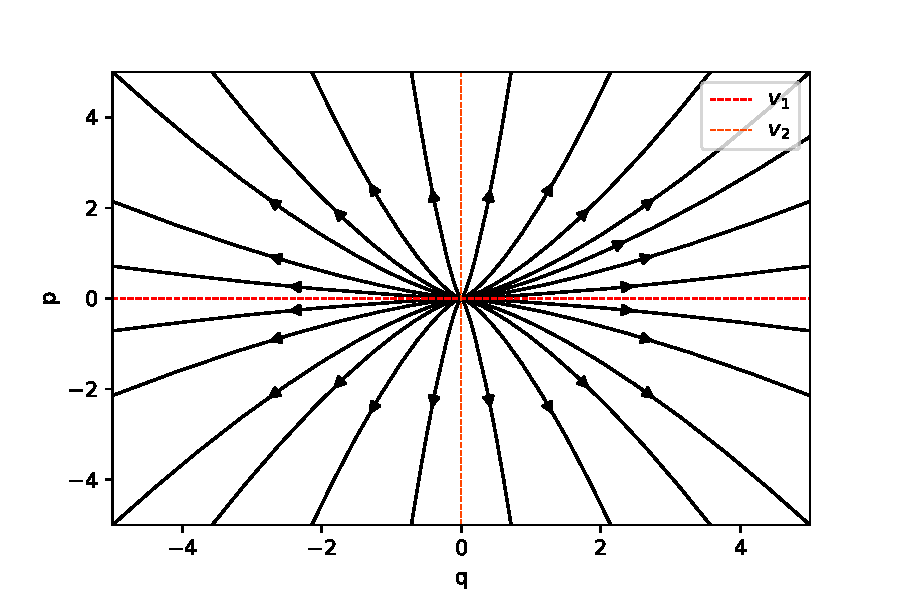
\includegraphics[scale=0.9]{punto-estable.pdf}
\caption{Nodo estable con autovectores $\vn_1=(1,0)$ y $\vn_2 = (0,1)$.}
\label{Fig:01-nodoestable}
\end{figure}

\newpage

\begin{figure}[h!] \centering
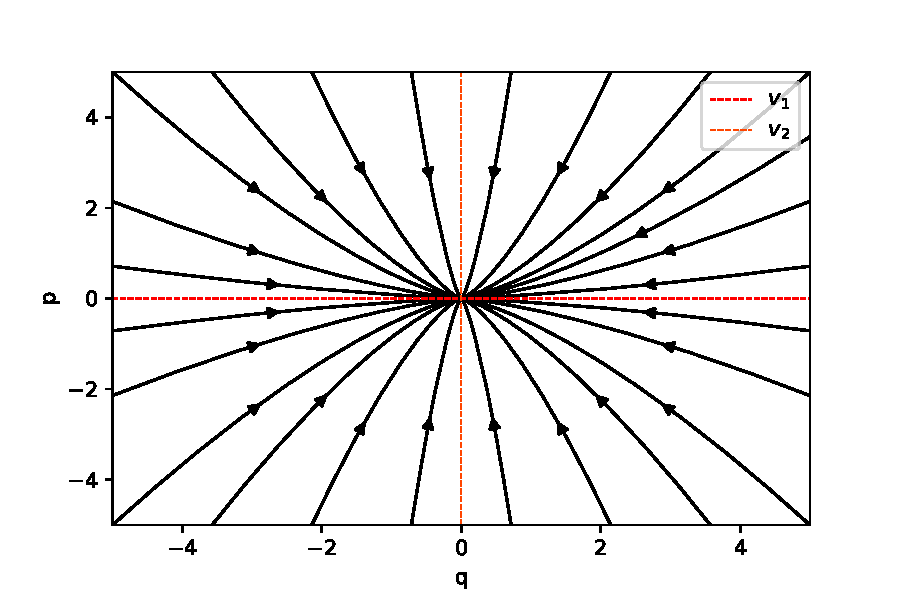
\includegraphics[scale=0.9]{punto-inestable.pdf}
\caption{Nodo inestable con autovectores $\vn_1=(1,0)$ y $\vn_2 = (0,1)$.}
\label{Fig:02-nodoinestable}
\end{figure}

\begin{figure}[h!] \centering
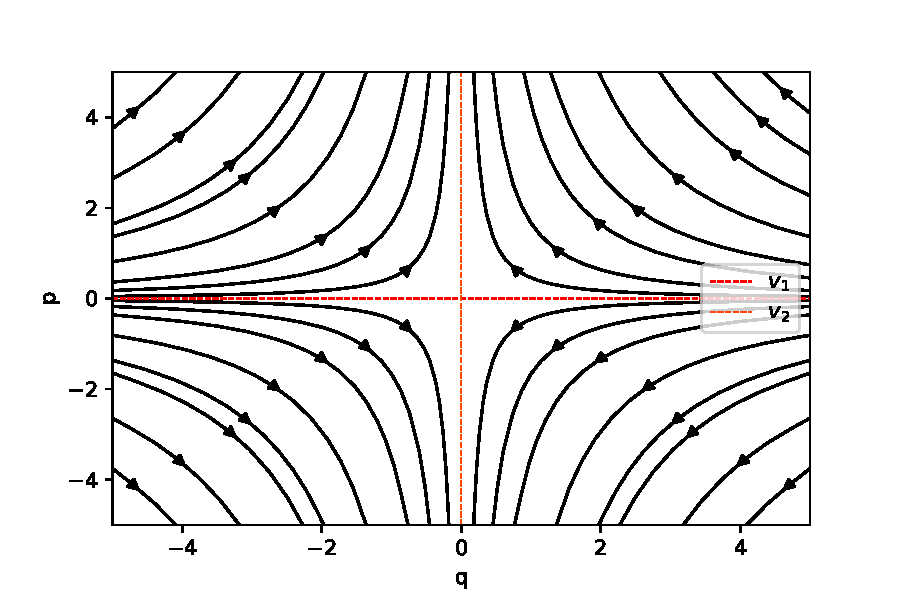
\includegraphics[scale=0.9]{punto-silla.pdf}
\caption{Punto silla con autovectores $\vn_1=(1,0)$ y $\vn_2 = (0,1)$.}
\label{Fig:03-puntosilla}
\end{figure}

\newpage

\begin{figure}[h!] \centering
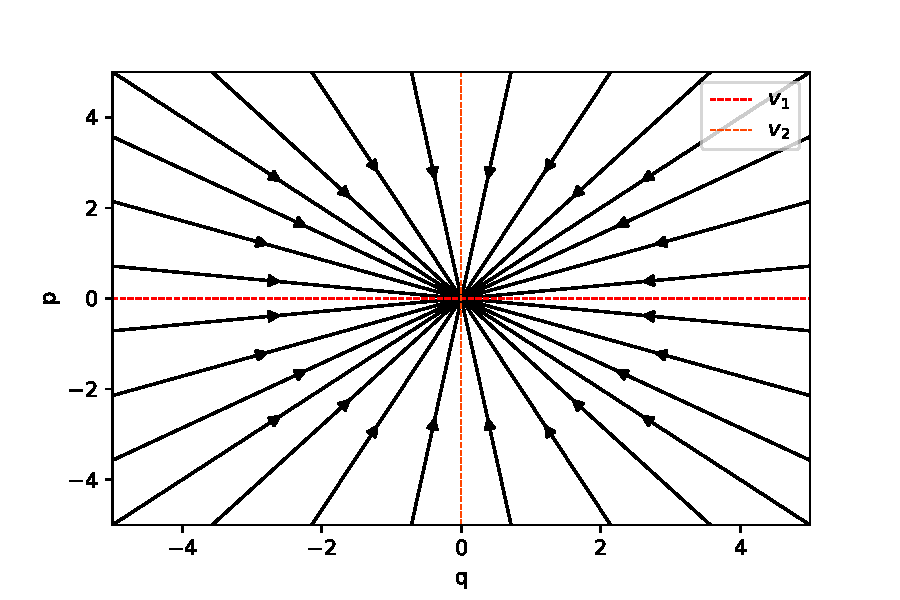
\includegraphics[scale=0.9]{nodo-dicritico-estable.pdf}
\caption{Nodo dicritico estable con autovectores $\vn_1=(1,0)$ y $\vn_2 = (0,1)$.}
\label{Fig:04-nodo-dicritico-estable}
\end{figure}

\begin{figure}[h!] \centering
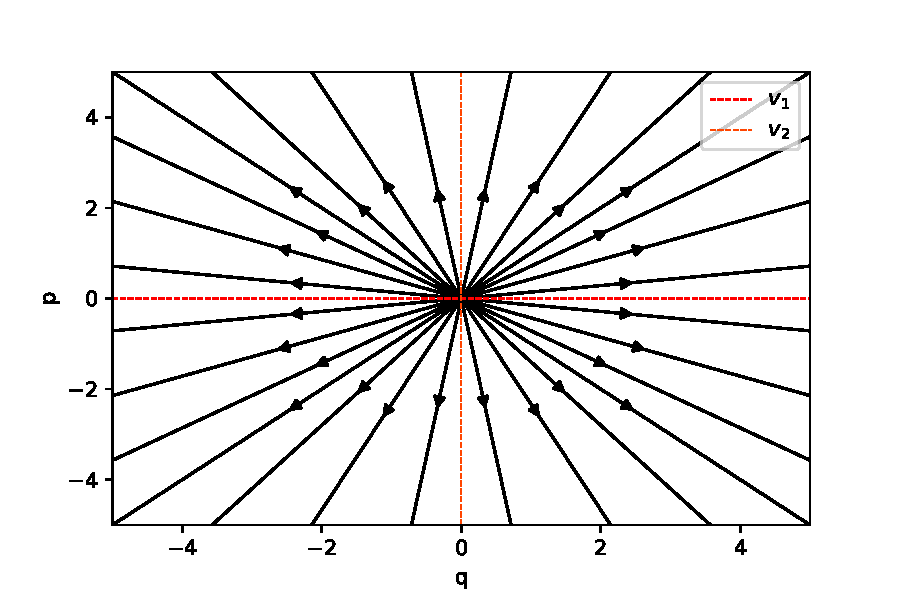
\includegraphics[scale=0.9]{nodo-dicritico-inestable.pdf}
\caption{Nodo dicritico inestable con autovectores $\vn_1=(1,0)$ y $\vn_2 = (0,1)$.}
\label{Fig:05-nodo-dicritico-inestable}
\end{figure}

\newpage


\begin{figure}[h!] \centering
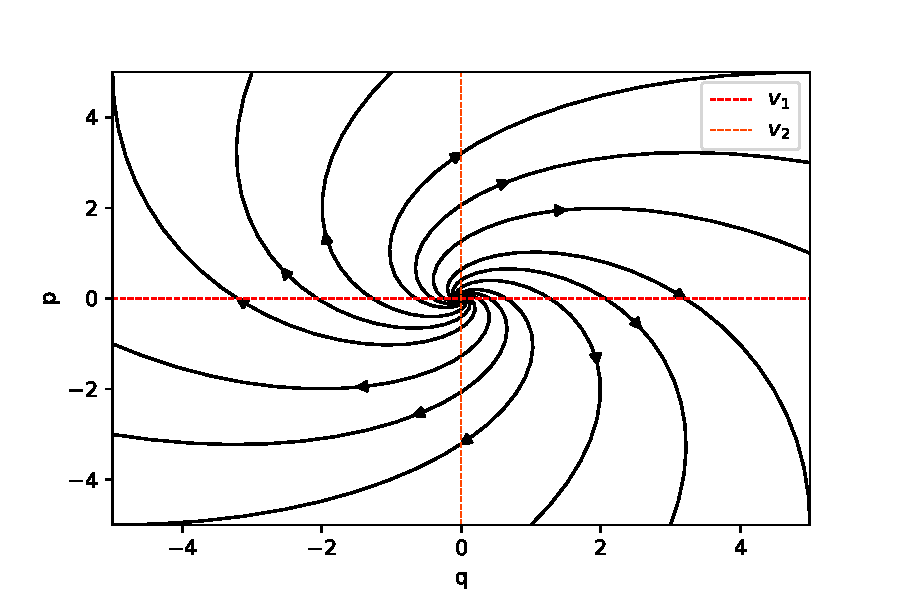
\includegraphics[scale=0.9]{nodo-inestable.pdf}
\caption{Foco inestable con autovectores $\vn_1=(1,0)$ y $\vn_2 = (0,1)$.}
\label{Fig:06-nodo-estable}
\end{figure}

\begin{figure}[h!] \centering
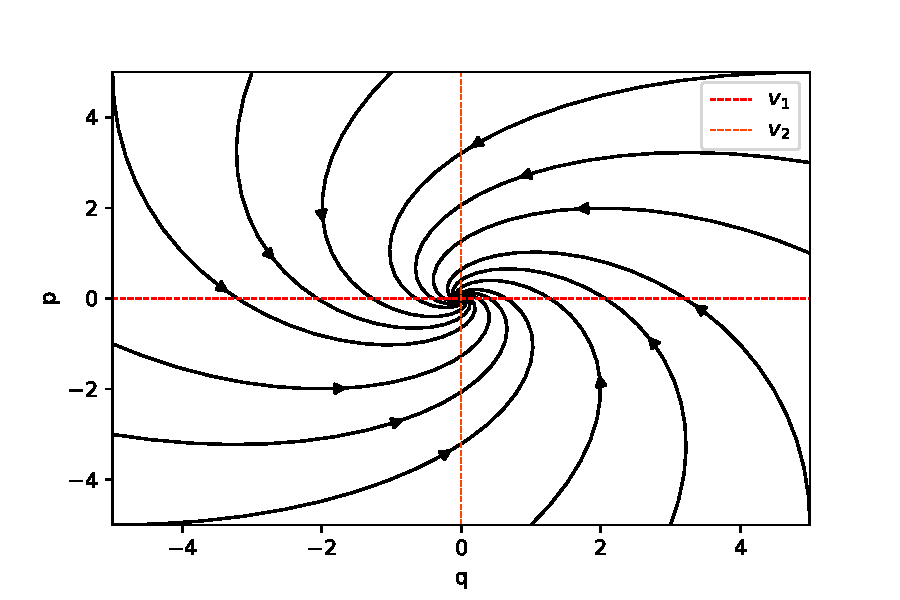
\includegraphics[scale=0.9]{nodo-estable.pdf}
\caption{Foco estable con autovectores $\vn_1=(1,0)$ y $\vn_2 = (0,1)$.}
\label{Fig:07-nodo-inestable}
\end{figure}


\newpage

\section{Medios Continuos}

Un medio continuo es un tipo de medio que puede ser estudiado dividiéndolo en celdas diferenciales, que sin ser moléculas o átomos, podemos entenderlas como partículas, con ciertas propiedades macroscópicas tales como la densidad, momento, temperatura... Cada una de estas celdas tendrá propiedades homogéneas (densidad homogénea en toda la celda, temperatura homogénea en toda la celda...). Esto es, cada celda estará en equilibrio termodinámico. Además podemos suponer entre dos celdas consecutivas las propiedades macroscópicas varían infinitesimalmente, de tal modo que la densidad en todo el espacio formado por dichas celdas es una función continua. \\


\subsection{Descripción euleriana y lagrangiana}

Ahora vamos a tratar quizás el punto mas relevante para entender lo que vamos a hacer después. Existen dos maneras de estudiar los medios continuos. Una de ellas consiste en estudiar las propiedades en función del punto del espacio y del tiempo y otra de ellas es estudiar las propiedades en función de la partícula y del tiempo. Esto dará pie a dos descripciones completamente análogas del medio. \\


La \textbf{descripción material} o \textbf{descripción lagrangiana} asocia a cada partícula un vector $\Xn$, que será la posición de la partícula/celda en el instante inicial $t_0$. Esto nos permite por ejemplo crear una función que nos permita asignar a cada partícula $\Xn$ una posición en el espacio, una densidad o una velocidad, de tal manera que

\begin{equation}
\xn \equiv \xn(\Xn,t) \tquad \vn \equiv \vn(\Xn,t) \tquad \rho \equiv \rho (\Xn,t)
\end{equation}
es como si tuviéramos un detector que sigue a cierta partícula midiendo en el instante $t$ dichas propiedades. Por ejemplo $\xn (\Xn,t)$ nos describe la posición de la partícula $\Xn$ en el instante $t$, mientras que $\vn (\Xn,t)$ la velocidad de la misma en el instante $t$. A las propiedades que medimos de esta forma las llamamos \textbf{propiedades materiales}. \\

La \textbf{descripción espacial} o \textbf{descripción euleriana} asociada a cada punto del espacio un vector $\xn$. Esto nos permite por ejemplo conocer con precisión cual es la densidad de dicho punto del espacio, o conocer cual es la partícula $\Xn$ que pasa por el punto $\xn$ en el instante $t$, de tal forma que:

\begin{equation}
\Xn \equiv \Xn (\xn,t) \tquad \rho^* \equiv \rho^* (\xn,t)
\end{equation}
en este caso es como si tuviéramos un detector que se encuentra fijo y midiéramos las propiedades de dicho punto. A estas propiedades las llamamos \textbf{propiedades espaciales}. El asterisco indica que tienen argumentos diferentes. En este caso $\Xn(\xn,t)$ nos dice que en la posición $\xn$ el instante $t$ esta pasando la partícula $\Xn$, mientras que $T^* (\xn,t)$ nos dice la temperatura de la posición $\xn$ en el instante $t$. 

\subsubsection{Analogía entre descripciones}

Ambas descripciones son completamente análogas, ya que conocer que partícula esta pasando por el punto $\xn$ en el instante $t$ ($\Xn (\xn,t)$) es igual que conocer en que posición $\xn$ se encuentra la partícula $\Xn$ en el instante $t$ ($\xn(\Xn,t)$). Realizar dicho cambio no es mas que un cambio del sistema de coordenadas, ya que para un instante $t$ fijo ambas descripciones son equivalentes. \\
\begin{equation}
\xn = \xn (\Xn,t) \Longleftrightarrow \Xn = \Xn (\xn,t)
\end{equation}

Con las propiedades materiales y las propiedades espaciales ocurre algo similar, ya que podremos expresar una propiedad material en la imagen euleriana y una propiedad espacial en la imagen lagrangiana. Si $P^*$ es la expresión en la forma euleriana y $P$ es la expresión en la forma lagrangiana:


\begin{equation}
P = P (\Xn,t) = P^*(\xn(\Xn,t),t) \Longleftrightarrow P^* = P^* (\xn,t) = P(\Xn(\xn,t),t)
\end{equation}


\subsubsection{Derivadas materiales y espaciales}

El caso de las derivadas materiales y espaciales es un caso curioso que requiere una espacial mención. Una \textbf{derivada material} mide la tasa de cambio de cierta propiedad de una partícula concreta. Su descripción mas natural se hace en la imagen lagrangiana. Sea la propiedad material $P$ tal que:

\begin{equation}
\dfrac{\Dd P(\Xn,t)}{\Dd t} \equiv \parciales{P(\Xn,t)}{t}
\end{equation}
donde $\frac{\Dd }{ \Dd t}$ es lo que llamamos el \textit{operador derivación material}. Por ejemplo la velocidad:

\begin{equation}
\vn (\Xn,t) =  \dfrac{\Dd \xn}{\Dd t} \equiv \parciales{\xn(\Xn,t)}{t}
\end{equation} Como podemos ver esto asigna un vector velocidad a cada partícula del espacio en un instante $t$, un vector tangente al movimiento. Esto se conoce en la literatura como \textit{campo de velocidades}.  \\

El caso de la \textbf{derivada espacial} mide la tasa de cambio de cierta propiedad en un punto concreto del espacio. Su descripción mas natural se hace en la imagen euleriana. Sea la propiedad $P^*=P(\Xn(\xn,t),t)$ espacial tendremos que la tasa de cambio se evaluará como:

$$ \parciales{P^*(\xn,t)}{t}$$
esta expresión no solo informa acerca de quién es la partícula que pasa en el instante $t$ por dicho punto, sino que en general se mide sobre partículas distintas que pasan en instantes de tiempo cercanos. \\


\subsubsection{Derivada material en coordenadas espaciales}

El estudio de las propiedades de un medio ya hemos dicho que podemos analizarlo desde dos perspectivas completamente análogas: la descripción en función de la celda o en función de la posición. Ahora bien, cuando uno quiere estudiar como se comportan las derivadas en una u otra descripción debe tener en cuenta que tanto la descripción de la posición en función de la partícula o la descripción de la partícula en función de la posición dependen explicitamente del tiempo, por lo que si queremos estudiar cierta derivada material en función de la posición tendremos que tener en cuenta que la partícula se mueve. \\

Para entenderlo mejor: si queremos saber cual va a ser la tasa de cambio de una propiedad de cierta partícula en función de la posición (imagen euleriana), tendremos que tener en cuenta dos factores; el primero la variación de dicha propiedad en la posición actual de la partícula (sería la variación estática) y el segundo la variación de dicha propiedad en la dirección en la que se desplaza la partícula (variación dinámica). Es obvio que tenemos que tener en cuenta ambos factores si queremos hallar la \textit{derivada material en la imagen euleriana}. Matemáticamente se dice que el \textit{operador derivación material en la imagen euleriana} es:

\begin{equation}
\dfrac{\Dd}{\Dd t} \equiv \parciales{}{t} + \vn \cdot \vec{\nabla}  \label{Ec:3.1.3.008}
\end{equation}
La derivada material de la propiedad euleriana $P^*(\xn,t)$ viene dada por

\begin{equation}
\dfrac{\Dd P^*}{\Dd t} \equiv \parciales{P^*}{t} + \vn \cdot \vec{\nabla} P^*
\end{equation}
Así tenemos que:

\begin{equation}
\dfrac{\Dd P}{\Dd t} = \parciales{P^*}{t} + \vn \cdot \vec{\nabla} P^*
\end{equation}



\subsection{Linea de corriente y flujo}

\begin{definition}[línea de flujo]
Una línea de flujo es la trayectoria física que describe una partícula en el espacio al moverse en el seno del medio continuo, siendo $t$ el parámetro de evolución:

\begin{equation}
\dfrac{\D x^i (t)}{\D t} = v^i ( \xn(t),t)
\end{equation}

\end{definition}


\begin{definition}[línea de corriente]
Una línea de corriente es una curva integral del campo instantáneo de velocidades. Por tanto, si fijamos el tiempo a $t=t_0$, con $\lambda$ como parámetro de evolución, una línea de corriente verifica que

\begin{equation}
\dfrac{\D x^i_c (\lambda)}{\D \lambda} = v^i ( \xn(\lambda)_c,t_0)
\end{equation}
\end{definition}

Si para un cierto flujo el campo de velocidades es independiente ddel tiempo, tenemos que \textit{la línea de flujo y la línea de corrientes coinciden}. 


\begin{definition}[línea de fluido]
Una línea de fluido es una línea material, y está constituida por todas las partículas que en un instante de tiempo formaron una curva en su evolución. Para ello basta con parametrizar una curva $X^i (\lambda)$ en el espacio de condiciones iniciales. Entonces

\begin{equation}
x^i_{fl} (\lambda,t_0)  = x^i (\Xn(\lambda),t_0)
\end{equation}
es la línea material a $t=t_0$ formada por las mismas partículas que en el instante inicial estaban en $X^i (\lambda)$. 
\end{definition}


\begin{definition}[línea de traza]
Una línea de traza es una curva espacial que une a todas las partículas emitidas sucesivamente desde un cierto punto. Para dar la forma analítica, debemos generalizar la expresión de una línea de flujo a tiempo inicial $\tau$ arbitrario

\begin{equation}
x^i = x^i (\Xn(\lambda),\tau,t)
\end{equation}

\end{definition}

\subsection{Variables de deformación}

\subsubsection{Deformación y desplazamiento}

El estudio de las variables de deformación es, sin lugar a dudas, la parte mas interesante, profunda y bonita de la mecánica del medio continuo y de los fluidos. Definimos \textbf{deformación} como la diferencia entre los configuraciones instantáneas (posiciones de cada partícula en los instantes $t=t_1$ y $t = t_2$). \\

Sea $t_1=0$ tal que la configuración inicial $x_i (\Xn,0)=X_i $ y la configuración final $x_i (\Xn,t)=x_i$ para $t_2=t$. Aquí lo que acabamos de hacer es definir las etiquetas de cada partícula como la posición en el instante inicial. Así podremos decir que $\Xn_j=(2,1,1)$ es la partícula que se encontraba en (2,1,1) en el instante $t_1$. Es interesante definir una aplicación entre dos configuraciones en instantes diferentes, llamada \textbf{desplazamiento} $u_i$ definida como

\begin{equation}
u_i = x_i - X_i 
\end{equation}
Pudiendo expresarse en la imagen lagrangiana o en la imagen euleriana

\begin{equation}
u_i (\Xn,t) = x_i (\Xn,t) - X_i \tquad u_i^* (\xn,t) = x_i - X_i (\xn,t) \label{Ec:3.3.1.013}
\end{equation}

Supongamos que estamos evaluando un desplazamiento infenitesimal, donde $t \longrightarrow \D t$, tendremos que $x_i$ se podrá desarrollar en su serie de Taylor centrado en $t=0$ tal que

\begin{equation}
x_i (\Xn,\D t ) = x_i (\Xn,0) + v_i (\Xn,0) \D t + (\cdots) 
\end{equation}
donde si despreciamos aquellos ordenes de magnitud mayores que 1 tendremos que el \textit{desplazamiento infenitesimal} será:

\begin{equation}
 u_i \cong v_i (\Xn,0) \D t \label{Ec:3.3.1.014}
\end{equation}
En la dinámica de fluidos, a diferencia de la dinámica de los sólidos, mucho mas aburrida, nos importa la historia entre dos configuraciones, por eso nos interesa llevar a la diferencia infenitesimal el desplazamiento. Lógicamente cuando $u_i$ no sea constante habrá una rotación o una deformación. Por esta misma razón estudiar la dependencia del desplazamiento respecto la posición 

\subsubsection{Gradiente de desplazamiento}

Ahora bien, esta velocidad podría depender de la partícula. Por eso creamos un \textbf{tensor gradiente de desplazamiento} $K_{ij}$, que nos da información de como varía el desplazamiento infinitesimal para cada partícula:

\begin{equation}
K_{ij} \equiv \parciales{u_i}{X_j}
\end{equation}
Supongamos que queremos describir este gradiente en función de la posición. Sabemos que $x_j (\Xn,t)$, por lo que:

\begin{equation}
K_{ij} = \parciales{u_i}{X_j} =\parciales{u_i}{x_k} \parciales{x_k}{X_j}   \label{Ec:3.3.2.017}
\end{equation}
donde ponemos el subíndice $k$ porque hay que tener en cuenta todas las coordenadas espaciales. Revisando la expresión \ref{Ec:3.3.1.013} podemos darnos cuenta que

\begin{equation}
\parciales{x_k}{X_j } = \parciales{(u_k + X_k)}{X_j} = \parentesis{\delta_{kj} + \parciales{u_k}{X_j}} \cong \delta_{kj}
\end{equation}
tal que hemos supuesto que las variaciones infenitesimales $\parciales{u_k}{X_j} \ll 1$. De esta forma es trivial que la ecuación \ref{Ec:3.3.2.017} genera la siguiente expresión:

\begin{equation}
K_{ij} \equiv \parciales{u_i}{X_j} = \parciales{u_i}{x_j}
\end{equation}

Ahora bien, esta no es la forma mas común de expresarla. La forma mas común de expresar el tensor gradiente de desplazamiento es usando dos tensores: el \textit{tensor tensiones} $\epsilon_{ij}$ y el \textit{tensor rotación} $\omega_{ij}$, tal que:

\begin{equation}
K_{ij} = \epsilon_{ij} + \omega_{ij} \tquad \epsilon_{ij} = \dfrac{1}{2} \parentesis{\parciales{u_i}{x_j} + \parciales{u_j}{x_i}}  \quad \omega_{ij} = \dfrac{1}{2}  \parentesis{\parciales{u_i}{x_j} - \parciales{u_j}{x_i}}
\end{equation}
¿Por qué expresarlo así? La razón por la cual se hace este cambio de variables no es obvia ni muchísimo menos. Esta es la forma para la cual el tensor gradiente de desplazamiento adquiere su significado físico mas interesante: el tensor tensiones nos dará una medida de como se comprime el fluido y el tensor rotación una medida de cuanto rota. Es decir, el tensor gradiente lo único que nos dice es hacia donde se desplazan las partículas del medio en función de su posición, pero no como lo hacen. Dichos dos tensores si que lo harán.  

\subsubsection{Deformación del elemento de volumen}

Una de las partes mas interesantes del medio continuo, a diferencia de un sólido, es que las partículas del medio pueden comprimirse o expandirse. Si suponemos un paralepipedo con coordenadas iniciales $\D \Xn^a$ (a=1,2,3), tal que el volumen viene dado por el doble producto escalar/vectorial expresado, pudiendo  expresarse con índices usando el operador levi-civita:

\begin{equation}
\D V_0 = \D \Xn^1 \cdot (\D \Xn^2 \times \D \Xn^3) = \epsilon_{ijk} \D X^1_i \D X^2_j \D X^3_k
\end{equation}

En un instante posterior estas aristas se habrán movido según la ecuación $\xn(\Xn,\D t)$, tal que si $\D t \ll 1$ tendremos que:

\begin{equation}
\D x_i ^a = \parciales{x_i}{X_j} \D X_j^a
\end{equation}
y por tanto el volumen en un instante $\D  t $ vendrá dado por:

\begin{equation}
\D V = \det \parentesis{\parciales{x_i}{X_j}} \D V_0
\end{equation}
donde $\parciales{x_i}{X_j}$ no es mas que el jacobiano del cambio de variables $\Xn \longrightarrow \xn$, lo cual tiene todo el sentido del mundo. Ahora bien, si estas son también infenitesimales, tendremos que: 

$$ \parciales{x_i}{X_j} = \delta_{ij}  + \parciales{u_i}{X_j} \cong \delta_{ij} + \parciales{u_i}{x_j} \longrightarrow  \det \parentesis{ \delta_{ij} + \parciales{u_i}{x_j}} = 1 + \parentesis{u_i}{x_i} $$
tal que:

\begin{equation}
\D V \cong \det \parentesis{\delta_{ij} + \parciales{u_i}{x_i}} \D V_0 = ( 1 + \Tr ( K)) \D V_0
\end{equation}
donde si tenemos que en cuenta que en la traza equivale a sumar aquellos $ij$ donde $i=j$ tal que $\omega_{ij} = 0$ eso nos indica que un movimiento de rotación \textit{no deforma el fluido} y que es el \textit{tensor de tensiones} el que nos da \textit{toda la información acerca de la deformación} del fluido.

\subsection{Ritmo de deformación y vorticidad}

No cabe duda que esto se ha hecho en general, sin embargo cuando tratamos con fluidos lo mas normal es aproximar al deformación a la velocidad, tal y como hemos hecho en la ecuación   \ref{Ec:3.3.1.014}. En ese caso tendremos que es el \textit{campo de velocidades} el que contiene información acerca del ritmo de deformación del fluido, lo cual es, de primeras, muy natural. Un fluido que está quieto o que su velocidad es igual para cualquier partícula nos podemos imaginar que no se deforma, que simplemente sigue un curso. Ahora bien, si la velocidad tiene direcciones/valores diferentes para cada partícula aparecen vórtices en el fluido, o simplemente aparecen zonas donde se apila el fluido. A partir de ahora definimos el \textbf{gradiente de velocidad espacial} $\mathcal{L}$ como:

\begin{equation}
\mathcal{L}_{ij} = \parciales{v_i}{x_j} = D_{ij} + W_{ij} \tquad D_{ij} = \dfrac{1}{2} \parentesis{\parciales{v_i}{x_j} + \parciales{v_j}{x_i}}  \quad W_{ij} = \dfrac{1}{2}  \parentesis{\parciales{v_i}{x_j} - \parciales{v_j}{x_i}}
\end{equation}
donde $D_{ij}$ será el \textbf{tensor de ritmo de deformación} y $W_{ij}$ es el \textbf{tensor ritmo de rotación} o \textbf{vorticidad}. 

\subsection{Derivadas material de elementos e integrales de volumen}

Observamos que $\D V(t)$ no es más que una propiedad material, ya que nos dice \textit{el volumen que ocupa una cantidad elemental de materia fija durante su evolución}. Por tanto tiene sentido preguntar cual es la derivada material:

\begin{equation}
\dfrac{\Dd (\D V(t))}{\Dd t} = \dfrac{\Dd J(t)}{\Dd t} \D V_0
\end{equation} 




\begin{lemma}
La derivada material del jacobiano de una matriz $\mathcal{F}(t)$ tal que  $J(t) = \det \mathcal{F}(t)$ viene dado por:
\begin{equation}
\dfrac{\Dd J}{\Dd t} = (\vec{\nabla} \cdot \vn) J(t)
\end{equation}
\end{lemma}

\begin{proff}
Por un lado tenemos que:
$$ \vec{\nabla} \cdot \vn = \parciales{v^i}{x^i} = \parciales{v^i}{X^k} \parciales{X^k}{x^i} = \parentesis{\parciales{}{X^k} \dfrac{\Dd x_i (\Xn,t)}{\Dd t}} \parciales{X^k}{x^i} = \dfrac{\Dd}{\Dd t} \parentesis{\parciales{x_i (\Xn,t)}{X^k}} \parciales{X^k}{x^i}; \quad \mathcal{F} = \parciales{x_i}{X_k} $$
$$ \vec{\nabla} \cdot \vn = \Tr \parentesis{\dfrac{\Dd \mathcal{F}}{\Dd t} \mathcal{F}^{-1}} = \dfrac{\D}{\D t} \parentesis{\Tr (\log \mathcal{F})} =  $$
si tenemos en cuenta la identidad matricial $\Tr (\log \mathcal{F}) = \log (\det \mathcal{F})$ implica que:
$$ \vec{\nabla} \cdot \vn = \dfrac{\Dd}{\Dd t} \log (J(t)) = \dfrac{1}{J(t)} \dfrac{\Dd J}{\Dd t} $$
\end{proff}
Entonces la derivada del volumen: 

\begin{equation}
\dfrac{\Dd (\D V)}{\Dd t} = (\vec{\nabla} \cdot \vn) J(t) \D V_0 =  (\vec{\nabla} \cdot \vn) \D V
\end{equation}

\subsubsection{Teorema de Transporte de Reynolds}

Supongamos que un volumen matricial se mueve con el medio y por tanto contiene siempre las mismas partículas. En ese caso las paredes siempre están formadas por los mismos elementos de fluido. Entonces si determinada propiedad $P(t)$ viene dada por la integral de volumen sobre cierta región material $V(t)$ a tiempo $t$:

\begin{equation}
P (t) = \int_{V(t)} p^* (\xn,t) \D^3 x = \int_{V_0} p (\Xn,t) J(t) \D^3 X
\end{equation} 

Ahora hay que tener en cuenta que la derivada temporal: 

$$ \dfrac{\Dd P(t)}{\Dd t} = \int_{V_0} \dfrac{\D}{\D t} \ccorchetes{p (\Xn,t) J(t)} \D^3 X  = \int_{V_0} \ccorchetes{\dfrac{\Dd p(\Xn,t)}{\Dd t} + p(\Xn,t) (\vec{\nabla} \cdot \vn) } J(t) \D^3 X  $$

Eso da cuenta del \textbf{teroema de transporte de Reynolds}, que básicamente nos da cual es la tasa de cambio de una propiedad material en un un volumen $V(t)$ en un instante $t$. Podemos escribirlo en función de la densidad $p^*(\xn,t)$ o de la densidad en la imagen lagrangiana $p(\Xn,t)$: 

\begin{equation}
\dfrac{\Dd [P(t)]}{\Dd t} = \int_{V(t)} \ccorchetes{\dfrac{\Dd p}{\Dd t} + p (\vec{\nabla} \cdot \vn)} \D^3 x \label{Ec:3.5.1.030}  
\end{equation}
\begin{equation}
\dfrac{\Dd [P(t)]}{\Dd t} = \int_{V(t)} \ccorchetes{\parciales{ p^*}{ t} +  \vec{\nabla} \cdot (p^* \vn)} \D^3 x \label{Ec:3.5.1.031}  
\end{equation}
donde hemos usado la expresión \ref{Ec:3.1.3.008}. Utilizando el teorema de Gauss vemos que esta expresión admite otra forma:

\begin{equation}
\dfrac{\Dd [P (t)]}{\Dd t} = \int_{V(t)} \parciales{p^*}{t} \D V + \int_{S(t)} p^* \vn \cdot \D \Sn
\end{equation}

A la magnitud $p^* \vn$ se denomina \textit{flujo} o \textit{corriente} asociada a la magnitud $P$. La segunda forma del Teorema de Reynolds hace trasparente las dos fuentes de variación de dicha magnitud en un cierto instante de tiempo. La primera contribución se debe a que la propia densida asociada pueda depender del tiempo y la segunda tiene un carácter cinemático y es proporcional a la corriente neta que atraviesa la superficie fronteriza.

\subsection{Dinámica de medios continuos}

El objetivo de la dinámica de medios continuos es establecer una serie de leyes de evolución capaces de predecir la evolución de un cierto sistema a partir de condiciones iniciales. Como el modelo estudiado se basa en la dinámica clásica, la piedra angular de la dinámica de los medios continuos será las segunda ley de Newton

\begin{equation}
m \dfrac{\D \pn}{\D t} = \Fn
\end{equation}

En el caso de los medios continuos existen varias leyes de conservación además de esta (en ausencia de fuerzas el momento lineal se conserva). En esta sección estudiaremos todas ellas.

\subsubsection{Conservación de la masa}

La magnitud que asocia la masa de un fluido con el volumen es la \textit{densidad de materia} $\rho (x)$. La masa total encerrada en un volumen es la integral:

\begin{equation}
m = \int_{V(t)} \rho (x) \D V
\end{equation}
si $V(t)$ es un volumen material, siempre contendrá las mismas partículas. La ley de conservación de la masa establece que la materia ni se crea ni se destruye, por lo que:

\begin{equation}
\dfrac{\Dd m}{\Dd t} = 0
\end{equation}
entonces según el teorema de transporte de Reynolds \ref{Ec:3.5.1.030} y \ref{Ec:3.5.1.031}, tendríamos que:

\begin{equation}
\int_{V(t)} \ccorchetes{\parciales{\rho}{t} + \vec{\nabla} \cdot (\rho \vn)} \D V = 0 \longrightarrow \parciales{\rho}{t} + \vec{\nabla} \cdot (\rho \vn) = 0  \label{Ec:3.6.1.036}
\end{equation}

Cuando la densidad de un volumen es constante decimos que el medio es \textit{incompresible}. En ese caso tendremos que $\rho (\xn,t) = \rho_0$

$$ \dfrac{\Dd \rho}{\Dd t} = 0 \longrightarrow \parciales{\rho}{t} + \vn \cdot \nabla (\rho) = 0 \longrightarrow \vn \cdot \nabla (\rho) - \nabla \cdot (\rho \vn) = 0  \longrightarrow \vec{\nabla} \cdot \vn = 0$$
de lo cual se deduce la otra forma de escribir la \textit{incompresibilidad de un fluido}:
\begin{equation}
\vec{\nabla} \cdot \vn = 0
\end{equation}

\subsubsection{Conservación del momento lineal}

La \textit{corriente de masa} $\rho \vn$ también se llama \textit{densidad de momento lineal}, y es generalización del momento lineal $m \vn$ de una partícula. Entonce el momento lineal de una cierta porción de materia $\Pn$ es

\begin{equation}
\Pn = \int_V \rho \vn \D V
\end{equation}
La generalización de la ecuación de Newton será:

\begin{equation}
m \dfrac{\D \pn}{\D t} = \Fn   \Longleftrightarrow \dfrac{\Dd}{\Dd t} \int_V \rho \vn \D V = \Fn
\end{equation}
Entonces si $\gn$ es la fuerza que actúa en cada partícula dentro del volumen $V(t)$ y $\fn_S$ es la fuerza por unidad de superficie que se ejerce en el contorno de $V(t)$. 

\begin{equation}
\dfrac{\Dd}{\Dd t} \int_V \rho \vn \D V = \int_V \rho \gn \D V + \int_S \fn_S \D S = \Fn_V + \Fn_S
\end{equation}


A la hora de estudiar la fuerza superficial lo que hacemos es suponer que $\fn_S$ no es mas que un tensor llamado el \textit{campo tensorial de esfuerzos} tal que $f_i \D S= \sigma_{ij} (\xn) n_j \D S$ donde la integral de superficie queda reducida a:

\begin{equation}
F_{S,i} = \int_S f_{S,i} \D S = \int_S \sigma_{ij} n_j \D S
\end{equation}
de tal forma que podamos aplicar el teorema de Gauss tal que:

\begin{equation}
F_{S,i} = \int_V  \parciales{\sigma_{ij}}{x_j} \D V
\end{equation}
Ahora bien, ¿Por qué suponemos que la fuerza superficial viene dado por un tensor llamado tensor de esfuerzos? Experimentalmente se debe a que todo medio continuo es capaz de trasmitir fuerzas de contacto a un punto vecino. Entonces una acción de contacto trasmite una fuerza $\fn_S$ sobre el medio a través de esta superficie, aunque no tiene por qué tener la misma dirección que la normal a la superficie $\hnn$. En ese caso decimos que si son paralelas hablamos de una fuerza de tensión/presión, o si son perpendiculares de fricción. Para dar cuenta de esto usamos un tensor, que nos dice como actúa parte del medio sobre otra contigua. Entonces expresando de manera diferencial, tenemos que la \textbf{ecuación de conservación del momento lineal} usando la ecuación \ref{Ec:3.6.1.036} queda en:

\begin{equation}
\rho \dfrac{\Dd v_i}{\Dd t} = \rho g_i + \parciales{\sigma_{ij}}{x^j} \tquad 
\end{equation}

\subsubsection{Conservación del momento angular}

En la definición del tensor de tensiones $\sigma_{ij}$ los índices juegan papeles diferentes, por lo que no hay ninguna razón para pensar que fuese simétrico. Sin embargo si estudiamos la conservación del momento angular llegamos a que para que se conserve dicho tensor debe ser simétrico. La generalización del momento angular en el medio natural:

\begin{equation}
\Ln = \int_V \xn \times \rho \vn \D V
\end{equation}
y si el torque es:

\begin{equation}
\Nn = \int_S \xn \times \fn_S \D S + \int_V \xn \times \rho \gn \D V
\end{equation}
implica que para que se conserve el momento angular:

\begin{equation}
\dfrac{\Dd \Ln}{\Dd t} = \Nn
\end{equation}
debe verificarse que $\sigma_{ij}=\sigma_{ji}$. 

\subsubsection{Conservación de la energía}

La conservación de la energía interna viene dada por las ecuaciones termodinámicas $\D U =\D W + \D Q$. En ese caso tenemos que si:

\begin{equation}
U = \int_V \rho u \D V
\end{equation}
siendo $u$ la \textit{densidad de energía interna}. Ahora bien, la variación de la energía interna de un volumen viene dada por la relación entre la deformación ($D_{ij}$) y el esfuerzo para deformar las partículas  ($\sigma_{ij}$). Además si tenemos en cuenta que a través de la superficie puede entrar una cantidad $\qn$ de calor (siendo este el flujo de calor), tendríamos que:

\begin{equation}
\dfrac{\Dd U}{\Dd t} = \int_V \sigma_{ij} D_{ij} \D V - \int_S \qn \D \Sn
\end{equation}
tal que de forma diferencial:


\begin{equation}
\rho \dfrac{\Dd u}{\Dd t} = \sigma_{ij} D_{ij} - \nabla \cdot \qn
\end{equation}
que sería el análogo del \textit{primer principio de la termodinámica} para los medios continuos. 



\subsection{Caracterización de medios continuos}


\subsubsection{Relaciones constitutivas}


Existen dos relaciones constitutivas (que no es mas que la relación de parámetros con otros parámetros) experimentales muy interesantes. Estas son:

\begin{itemize}\item La relación entre el tensor de esfuerzos con el tensor de deformaciones ($\epsilon_{ij}$) y el ritmo de deformaciones ($D_{ij}$). En ese caso:

\begin{equation}
\sigma_{ij} = \sigma_{ij} (\epsilon,D)
\end{equation}
\item La \textit{ley de Fourier} nos relaciona el flujo de calor con el gradiente de una función escalar llamada temperartura a través de una constante $\kappa$ llamada \textit{conductividad térmica}:

\begin{equation}
q_i = - \kappa \parciales{T}{x_i}
\end{equation}
\end{itemize}

\subsubsection{Ecuaciones del movimiento}

Teniendo en cuenta esto vamos a escribir todas las ecuaciones del movimiento de los medios continuos:

\begin{itemize}
\item \textbf{Ecuación de continuidad}:
\begin{equation}
\dfrac{\Dd \rho}{\Dd t} = - \rho \vec{\nabla} \cdot \vn
\end{equation}
\item \textbf{Conservación del momento lineal}:
\begin{equation}
\rho \dfrac{\Dd v_i}{\Dd t} = \parciales{\sigma_{ik}}{x_k} + \rho g_i
\end{equation}
\item \textbf{Conservación de la energía}:
\begin{equation}
\rho \dfrac{\Dd u}{\Dd t} = \sigma_{ij} D_{ij} + k \Delta T
\end{equation}
\item \textbf{Ecuación constitutiva}:
\begin{equation}
\sigma_{ij} = \sigma_{ij} ( \epsilon , \D)
\end{equation}
\item \textbf{Ecuación termodinámica}:
\begin{equation}
T = T (s,\epsilon ,D)
\end{equation}
\end{itemize}
donde $\Delta$ es el laplaciano y $s$ la densidad de entropía.

\newpage



\section{Fluidos}

\subsection{Fluido Newtoniano}

Trabajar con las ecuaciones del movimiento tal y como las hemos expresado es un tanto imposible sin estudiar experimentalmente un medio, ya que necesitamos conocer  una forma funcional aproximada de los tensores de esfuerzos, tensor de de deformaciones... Muchos de los medios tienen comportamientos generales muy parecidos entre sí. Este es el caso de los \textit{fluidos Newtonianos}, donde entran aire, agua...  Ahora vamos a tratar de escribir los axiomas de los fluidos:

\begin{itemize}
\item \textit{Ausencia de esfuerzos cortantes:} en estado de reposo el fluido no soporta esfuerzos constantes, de tal modo que en reposo $\sigma_{ij} = - p \delta_{ij}$
\item \textit{Linealidad}: el tensor de esfuerzos solo depende del ritmo de deformación siendo lineal esta dependencia:

\begin{equation}
\sigma_{ij} = - p \delta_{ij} + c_{ijkl} Y_{kl}
\end{equation}

\item \textit{Simetría}: una rotación rígida no ocasiona ningún tipo de esfuerzo interno, por lo que $Y_{kl}=D_{kl}$. 

\item \textit{Isotropía}: no hay ningún tipo de dirección privilegiada del movimiento, por lo que $c_{ijkl}$ vienen dadas por funciones escalares. 
\end{itemize}

Eso leva a pensar que el fluido newtoniano verifica que:

\begin{equation}
\sigma_{ij} = (-p + \lambda \vec{\nabla} \cdot \vn) \delta_{ij}  + \mu \parentesis{\parciales{v_i}{x_j} + \parciales{v_ j}{x_i}} \label{Ec:4.1.0.002}
\end{equation}
donde $\lambda$ y $\mu$ son lo que llamamos \textit{viscosidad de volumen} y la \textit{viscosidad cortante}.

\subsection{Ecuación de Navier-Stokes}

En ese caso si despejamos las ecuaciones de continuidad para un fluido Newtoniano que verifica la ecuación \ref{Ec:4.1.0.002} tendremos 7 ecuaciones con 7 incógnitas: $p$, $\rho,$ $\vn$, $u$ y $T$, dadas por:

\begin{equation}
\begin{array}{rl}
\dfrac{\Dd \rho}{\Dd t} & =  \ - \rho \vec{\nabla} \cdot \vn \\ \\
\rho \dfrac{\Dd \vn}{\Dd t}  & = \  - \nabla p + (\lambda+ \mu) \nabla (\nabla \cdot \vn) + \mu \Delta \vn + \rho \gn \\ \\
\rho \dfrac{\Dd u}{\Dd t} &  = \ - p \nabla \cdot \vn + \lambda ( \nabla \cdot \vn)^2  + \mu \parentesis{\parciales{v_i}{x_j} + \parciales{v_j}{x_i}} \parciales{v_i}{x_j} + \kappa \Delta T \\ \\
p  & = \  p(u,\rho) \\ \\
T & =  \ T(u,\rho) 
\end{array}
\end{equation}

Ahora vamos a presentar los fluidos mas comunes:


\subsubsection{Fluido no-viscoso}

Imponemos que $\lambda = \mu = 0$. En ese caso las ecuaciones de Navier-Stokes son muchísimo mas sencillas:

\begin{equation}
\begin{array}{rl}
\dfrac{\Dd \rho}{\Dd t} & =  \ - \rho \vec{\nabla} \cdot \vn \\ \\
\rho \dfrac{\Dd \vn}{\Dd t}  & = \  - \nabla p + \rho \gn \\ \\
\rho \dfrac{\Dd u}{\Dd t} &  = \ - p \nabla \cdot \vn + \kappa \Delta T \\ \\
p  & = \  p(u,\rho) \\ \\
T & =  \ T(u,\rho) 
\end{array}
\end{equation}
Si además el fluido no tiene conductividad térmica ($\kappa = 0$):

\begin{equation}
\begin{array}{rl}
\dfrac{\Dd \rho}{\Dd t} & =  \ - \rho \vec{\nabla} \cdot \vn \\ \\
\rho \dfrac{\Dd \vn}{\Dd t}  & = \  - \nabla p + \rho \gn \\ \\
\rho \dfrac{\Dd u}{\Dd t} &  = \ - p \nabla \cdot \vn  \\ \\
p  & = \  p(u,\rho) \\ \\
T & =  \ T(u,\rho) 
\end{array}
\end{equation}


\subsubsection{Fluido incompresible}

Un fluido incompresible tal y como hemos visto es aquel que verifica que $\rho = \rho_0$ constante, de tal modo que:


\begin{equation}
\begin{array}{rl}
 \vec{\nabla} \cdot \vn & = \ 0 \\ \\
\rho \dfrac{\Dd \vn}{\Dd t}  & = \  - \nabla p +  \mu \Delta \vn + \rho \gn \\ \\
\rho \dfrac{\Dd u}{\Dd t} &  = \  \mu \parentesis{\parciales{v_i}{x_j} + \parciales{v_j}{x_i}} \parciales{v_i}{x_j} + \kappa \Delta T \\ \\
p  & = \  p(u,\rho) \\ \\
T & =  \ T(u,\rho) 
\end{array}
\end{equation}

\subsubsection{Otros}

El caso de un \textit{fluido estático} tendrá que $\vn = 0$. El caso de un \textit{fluido estacionario} tendrá que $\vn$ no depende de $t$. El caso de un \textit{fluido potencial} verifica que $\omega = \rota \vn = 0$, y por tanto podemos escribir $\vn$ como el gradiente de un campo escalar.

\subsection{Teorema de Bernoulli}

\begin{theorem}[Teorema de Bernoulli]
en un fluido no viscoso sometido a fuerzas conservativas donde $\gn = - \nabla \Omega$, donde el flujo es estacionario ($\vn$ no depende de $t$) verifica que la magnitud $B_1$ es constante en el tiempo:

\begin{equation}
B_1 = \int \parentesis{ \dfrac{\D p}{\rho} } + \dfrac{1}{2}v^2 + \Omega
\end{equation}
y si el flujo no es estacionario pero si potencial $\vn  = - \nabla \Phi$ se conserva la cantidad $B_2$:

\begin{equation}
B_2 = \parciales{\Phi}{t} + \int \parentesis{ \dfrac{\D p}{\rho} } + \dfrac{1}{2} (\nabla \Phi)^2 + \Omega
\end{equation}
integradas en una linea de corriente.

\end{theorem}

\end{document}
